\documentclass[journal]{IEEEtran}
%
% If IEEEtran.cls has not been installed into the LaTeX system files,
% manually specify the path to it like:
% \documentclass[journal]{../sty/IEEEtran}





% *** CITATION PACKAGES ***
%
\usepackage{cite}
% cite.sty was written by Donald Arseneau
% V1.6 and later of IEEEtran pre-defines the format of the cite.sty package
% \cite{} output to follow that of the IEEE. Loading the cite package will
% result in citation numbers being automatically sorted and properly
% "compressed/ranged". e.g., [1], [9], [2], [7], [5], [6] without using
% cite.sty will become [1], [2], [5]--[7], [9] using cite.sty. cite.sty's
% \cite will automatically add leading space, if needed. Use cite.sty's
% noadjust option (cite.sty V3.8 and later) if you want to turn this off
% such as if a citation ever needs to be enclosed in parenthesis.
% cite.sty is already installed on most LaTeX systems. Be sure and use
% version 5.0 (2009-03-20) and later if using hyperref.sty.
% The latest version can be obtained at:
% http://www.ctan.org/pkg/cite
% The documentation is contained in the cite.sty file itself.



\usepackage{array,tabularx,hyperref,tikz,enumitem}
\usetikzlibrary{shapes.geometric,shapes.arrows,decorations.pathmorphing}
\usetikzlibrary{matrix,chains,scopes,positioning,arrows,fit}
\usepackage[margin=1in]{geometry}


% *** GRAPHICS RELATED PACKAGES ***
%
\ifCLASSINFOpdf
  \usepackage{graphicx}
  % declare the path(s) where your graphic files are
  \graphicspath{ {Images/} }
  \usepackage[justification=centering]{caption}
  % and their extensions so you won't have to specify these with
  % every instance of \includegraphics
  % \DeclareGraphicsExtensions{.pdf,.jpeg,.png}
\else
  % or other class option (dvipsone, dvipdf, if not using dvips). graphicx
  % will default to the driver specified in the system graphics.cfg if no
  % driver is specified.
  % \usepackage[dvips]{graphicx}
  % declare the path(s) where your graphic files are
  % \graphicspath{{../eps/}}
  % and their extensions so you won't have to specify these with
  % every instance of \includegraphics
  % \DeclareGraphicsExtensions{.eps}
\fi






% *** MATH PACKAGES ***
%
\usepackage{amsmath,float}


\begin{document}
\title{Campus Location Recognition using {Audio~Signals}}

\author{James~Sun,Reid~Westwood
        \\
        SUNetID:{jsun2015,rwestwoo}\\
        Email: \href{mailto:}{jsun2015@stanford.edu},  \href{mailto:}{rwestwoo@stanford.edu} }


% make the title area
\maketitle




\section{Introduction} \label{Intro}
Recognizing one's location by sound is a coarse skill that many people seem to develop out of routine. We may be able to recognize a favorite caf\'e by the genre of music playing and the baristas' voices. We may be able to recognize the inside of our car by the noises coming out of the engine and chassis. We might come to associate the sounds coming through our rooms' windows with home. However, are these sounds by themselves truly sufficient to identify the locations that we frequent?
This project attempts to answer that question by developing a Machine Learning system that recognizes geographical location purely based on audio signal inputs. To emulate a typical Stanford student, the system is trained on sounds at locations along a path that a student might take as he or she goes about a typical school day. In the process of developing this system, we investigated audio features in both the spectral and time domain as well as multiple supervised learning algorithms.

\section{Related Work} \label{Related}
A previous CS229 course project identified landmarks based on visual features \cite{Crudge:article_typical}. \cite{Chen} gives a classifier that can distinguish between multiple types of audio such as speech and nature. \cite{Chu} investigates the use of audio features to perform robotic scene recognition. \cite{Chu2Env} integrated Mel-frequency cepstral coefficients (MFCCs) with Matching Pursuit (MP) signal representation coefficients to recognize environmental sound. \cite{guo2003content} uses Support Vector Machines (SVMs) with audio features to classify different types of audio.

\section{Scope}
As stated in Section \ref{Intro}, we have limited the number of areas that the system will recognize. Furthermore, we have limited the geographical resolution of labels to named locations encompassing areas such as Rains Graduate Housing. Both of these limitations are in line with how a typical person may use audio cues to identify his or her location. As such, these geographical restrictions in scope are unlikely to be relaxed.

We have also initially limited our scope temporally to data gathered on weekdays between the periods of 9AM to 5PM during the Spring Academic Quarter. Initial results are promising, and we may relax some of these restrictions.

\section{System Design}\label{SystemDesign}
\subsection{Hardware and Software}\label{HwSw}
The system hardware consists of an Android phone and a PC. The Android phone runs the Android 6.0 Operating system and uses the \texttt{HI-Q MP3 REC (FREE)} application to record audio. The PC uses Python with the following open-source libraries:
\begin{itemize}
\item Scipy
\item Numpy
\item statsmodels
\item scikits.talkbox
\item sklearn
\end{itemize}
The system also makes use of a few custom libraries developed specifically for this project.

\subsection{Signal Flow}\label{Signal Flow}
The following details the flow of a signal when making a prediction
\begin{enumerate}
\item Audio signal is recorded by the Android phone
\item Android phone encodes the signal as a Wav file
\item The Wav file enters the Python pipeline as a \texttt{Sample} instance
\item A trained \texttt{Classifier} instance receives the \texttt{Sample}
\begin{enumerate}
\item The \texttt{Sample} is broken down a number of subsamples based on a predetermined audio length for each subsample
\item A prediction is made on each subsample
\item The most frequent subsample prediction is output as the overall prediction.
\end{enumerate}
\end{enumerate}
A graphical illustration of this is below:\\


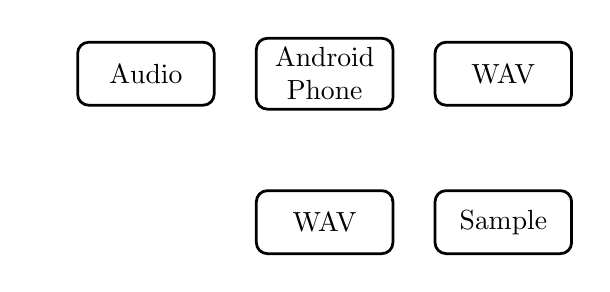
\begin{tikzpicture}
\matrix (m) [matrix of nodes, 
    column sep=5mm,
    row sep=1cm,
    nodes={draw, % General options for all nodes
      line width=1pt,
      anchor=center, 
      text centered,
      rounded corners,
      minimum width=1.5cm, minimum height=8mm
    }, 
        % Define styles for some special nodes
        right iso/.style={isosceles triangle,scale=0.5,sharp corners, anchor=center, xshift=-4mm},
        left iso/.style={right iso, rotate=180, xshift=-8mm},
        txt/.style={text width=1.5cm,anchor=center},
        ellip/.style={ellipse,scale=0.5},
        empty/.style={draw=none}]
    {
      % First row of symbols (mostly empty, only the power meter at the right end)
        % m-1-1 empty
      & |[txt]| {Audio}
      & |[txt]| {Android Phone}
      & |[txt]| {WAV}\\
      & % m-1-6 empty
      & |[txt]| {WAV}
      & % m-1-7
        |[txt]| {Sample} 
      \\
      };
\end{tikzpicture}
\subsection{Locations}
The system is trained to recognize the following 7 locations:
\begin{enumerate}[label=\arabic*.]
\addtocounter{enumi}{-1}
\item Arrillaga Gym
\item Bytes Caf\'e
\item Circle of Death
    \subitem Intersection of Escondido and Lasuen
\item Huang Lawn
\item The Oval
\item Rains Graduate Housing
\item Tressider Memorial Union
\end{enumerate}
These locations represent the route a typical graduate engineering student living at Rains might take on a typical day. Locations 0,1, and 6 are indoors whereas Locations 2,3,4, and 5 are outdoors.


\section{Data Collection}\label{Data}
\subsection{Format}
Data is collected using the \texttt{HI-Q MP3 REC (FREE)} application as noted in Section \ref{HwSw}. This application is freely available on the Google Play Store. Monophonic Audio is recorded without preprocessing and postprocessing at a sample rate of 44.1 kHz. 
\subsection{Training Data}
Training data is gathered during weekdays in the morning in order

\section{Methods}
The goal is to have the system recognize natural geographic aggregates rather than recognize individual fine-grain coordinates. For example, the system will label a data set as belonging to "The Quad" or "Bytes Cafe", similar to how a person would naturally describe an environment. I expect to use supervised learning algorithms to separate data points based on audio and visual features.
\subsection{Audio Features}
As audio is potentially the more interesting data type, I have come up with a few basic features to evaluate. These include the following:
\begin{itemize}
\item Frequency Spectrum Bandwidth
\item Frequency Spectrum Variance
\item Frequency Spectrum mean
\item Intensity variance
\item Mean Intensity
\end{itemize}

% references section

% can use a bibliography generated by BibTeX as a .bbl file
% BibTeX documentation can be easily obtained at:
% http://mirror.ctan.org/biblio/bibtex/contrib/doc/
% The IEEEtran BibTeX style support page is at:
% http://www.michaelshell.org/tex/ieeetran/bibtex/
%\bibliographystyle{IEEEtran}
% argument is your BibTeX string definitions and bibliography database(s)
%\bibliography{IEEEabrv,../bib/paper}
%
% <OR> manually copy in the resultant .bbl file
% set second argument of \begin to the number of references
% (used to reserve space for the reference number labels box)
\bibliographystyle{IEEEtran}
\bibliography{CS229_Progress_report}
\raggedbottom



\end{document}
